%System Design

\chapter{Design} % Main chapter title

This chapter provides a detailed description of the designed system. In section ~\ref{gfd}, the general framework design diagram is presented, along with a simplifying description of each module the diagram contains. 


\section{General Framework Design}
\label{gfd}
\begin{figure}
	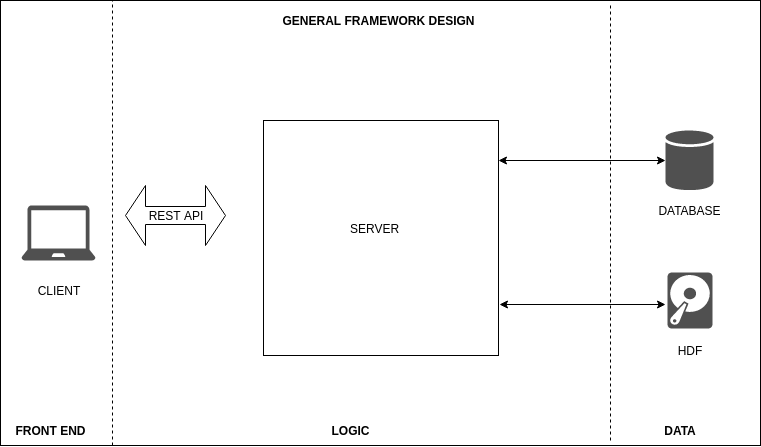
\includegraphics[scale=0.5]{framework.png}
	\caption{General Framework Design}
	\label{framework}
\end{figure}
In figure~\ref{framework} a general framework design diagram is presented. The system architecture is divided in three parts: front-end/presentation tier, logic tier and data tier, as described in chapter~\ref{3tierarch}. The data tier contains the database where all model data is stored, and the filesystem in which all uploaded datasets are saved in hdf form. The logic tier contains all the modules necessary for ensuring the framework functionality, such as crud operations, database access, authentication, authorization etc. The communication between logic and presentation tier is established over a rest api service. In the presentation tier, the user may interact with the server by sending requests and retrieve JSON data as responses.

\section{Generic Framework Modules}
In this section the framework modules used in this thesis are presented in detail. Diagrams are shown in some of these subsections for better understanding of the framework design. The modules are divided in four big categories: nosql access,user management, server and user interface. All modules and submodules are developed in a generic way, are highly customizable, extendible and reusable. This gives us the opportunity to often refer to these modules as models, as described in chapter~\ref{mdsd}. The level of abstraction may change, but the main characteristics of model driven software development are common in the framework implementation. Also, all modules are isolated and expose only the methods that must be used in the rest of the framework.


\subsection{Nosql access}
\begin{figure}
	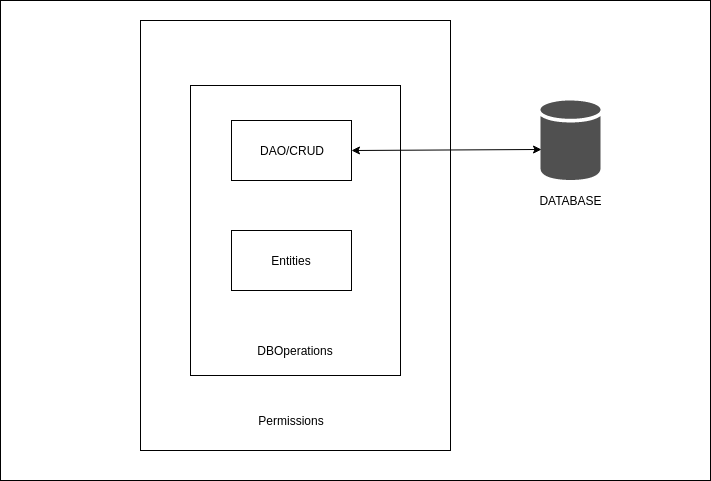
\includegraphics[scale=0.5]{nosqlaccess.png}
	\caption{Nosql access module structure}
	\label{nosqlaccess}
\end{figure}
The nosql access module is a very important component of the framework. It is responsible for a big part of the system's functionality, such as schema creation, CRUD operations generation, communication between server and database etc. As a result of its importance, this module is used as a dependency in many other models of the framework. This model is developed in such a way, so its functionality is isolated from the rest of the framework. Aside from the fact that this practice applies to the model-driven approach, it is generally a clean way for developing frameworks. The structure of the module can be seen in figure ~\ref{nosqlaccess}. Nosql access module consists of many submodules and each of those is presented separately below. 

\subsubsection{Entities}
\label{entities}
An entity is a representation of a database resource. The creation of an entity through our framework, corresponds to the creation of a collection in our database. Likewise, the creation of an instance of an entity, corresponds to the creation of a document inside a collection in our database. In this way it becomes very easy to make changes to the database, without having direct access to it, which is crucial for our framework.\par
	In the entities module, we define the entities we are going to use in the framework. More specific, we define the structure of the entities we use, their fields, their fields type, as well as the fields restrictions. For example, we can define if a field must be unique in relation with the rest of the instances in the same collection of the database. The definition of the entities is written in JSON form, so it becomes really easy to change or add more entities in the database. So, this module obtains the property of extensibility, which is really important for the model-driven architecture we created. \par 
	For the purpose of the application demo, we defined a list of entities with specific fields, field types and restrictions. A visualization of this list is shown in figure MPLAAAAA. An analysis of each of the entities can be seen below.\par
	
	 
\subsubsection{Users}
In order to use the application, a user is obligated to create a new user account. The necessary properties to create a new account are username, full name, password and email. Username and email must have unique values in relation with all other user instances. The entity Users contains all necessary fields to save the above information, in the addition of a unique id.
\subsubsection{Projects}
A basic concept of the application is the project entity. The application users may create new projects, in which multiple users may participate. The content of a project is visible for all users that participate in it. The required fields for the creation of a project instance are name, date and description. The project entity uses the concept of ACL, as described in chapter~\ref{acl}. Thus, project entity contains information about which users can or cannot, use a CRUD operation for the specific instance of the project entity. This way, the fields that contain this information reference an instance of a user entity.
\subsubsection{Datasets}
Another usefull entity of the application is Datasets. The application users may create their own datasets inside a project they participate. In this entity are saved the metadata of an hdf file which was uploaded on the application. The fields of this entity are the dataset name, date, a reference to the user instance who creates the entity, and the hdf filename. Also, a project instance reference,in which the dataset is in, is saved. Last, just as in project entity, information is retained about the access control list of the dataset.
\subsubsection{Posts}
An application user may create a new post inside a project. The required fields for the creation of a post entity are title, description, date, a dataset instance reference and a project instance reference. Also, acl information  is saved in the post entity instance. The user may create a post in response of another post. In that case, information is retained about the post instance in reference.
\subsubsection{Plots}
A user may add plots inside his posts. The required fields for the creation of a post entity are title, description, the path inside the hdf file in which the array used for the plot is saved, and the post instance reference. Also, the plot entity retains information about its metadata, such as plot type and the dimention values used in the plot.

\subsubsection{Data Access Object/ CRUD}
\label{daocrud}
As described in chapter~\ref{dao}, DAO provides some specific data operations without exposing details of the database which are not needed. In our case, the dao model ensures that it is the only module with access in the database, and exposes only the information and CRUD functions which are vital for the rest of the framework. The dao module is developed in a generic way and it is customizable by the entities module. Thus, for each of our entities, we generate CRUD operations for interaction between the specific database model and the framework. The CRUD methods used in the dao module are described in detail below.

\subsubsection{createItem}
The method createItem is responsible for the creation of new instances of an entity. It receives an object as an argument, it converts it in model instance form and then saves it. If an error occures, it returns a new Error object. Based in the single responsibility principle, the method does not control the kind of data that are about to be saved.
\subsubsection{readItems}
The method readItems is used to read data from the database. It receives a query object as an input. The result, successfull or not, is returned as an array object. If an error occures, it returns a new Error object.
\subsubsection{updateItem}
The method updateItem is responsible for updating an existing object in the database. To achieve that, it receives as arguments a query object and an object with the new property values. If found, the object is replaced and returned. If an error occures, it returns a new Error object.
\subsubsection{deleteItem}
The method deleteItem is used to delete an existing document from the database. It receives a query object as an input, and if the document is found, the method deletes it from the database. If an error occures, it returns a new Error object.

\subsubsection{DbOperations}
As mentioned in the section~\ref{daocrud}, the DAO module is responsible for interacting with the database. The model methods are interacting with the database, perform direct changes and may return a result where applicable. But is there a way to guarantee the integrity of our operations in live data? Throughout our study, we determined that all functions must be wrapped in functions responsible for the verification and validation of the requested data mutation. So in essense, we provide a single sandboxed environment securing the database from malicious adversaries, as well as potential internal missuse. \par 
	The DBOperations model was developed for this purpose. It receives as an argument the entities and the dao models. The DBOperations model returns a group of functions which control the data they receive as an input and then call the corresponding dao model methods. \par 
	The verification of the data is essential for the CRUD operations. In our case we primarily check if all the required properties and references are contained in the input object. Then, we verify that the references values are valid id's of the corresponding entities instance. In order to achieve that, the necessary read operations in the database are made.
	
\subsubsection{Permissions}
In chapter~\ref{entities}, we described that most of the entities contain some fields that are responsible for the accesss control list. To be able to alter these fields in relation with who can access or not a resource, we developed a module specialized for this task. This module contains some functions which implement the acl functionality. The dependencies of permissions model are entities and DBOperations models. \par 
	The Permissions modules defines all the roles the framework uses. At anytime we can add or remove a role, therefore the model-driven design approach is implemented. This model is also responsible for the verification of the changes that it is about to make. The module exposes only the desired methods, so that any unwanted functionality is isolated. The generic methods we developed are described below. 

\subsubsection{addUserRole}
This method adds a specific role to a user for the given resource. It receives four arguments as an input, the user id, the object id, the role and the model name. All arguments are verified before proceeding with the entity instance update.
\subsubsection{removeUserRole}
RemoveUserRole is a method that does the opposite of the addUserRole. It removes from a user a certain role of a resource. It also receives the same arguments as an input. All arguments are verified before proceeding with the entity instance update.
\subsubsection{isAllowed}
This method is the core of the acl logic. Its purpose is to check if  a user has the permission to perform a crud operation in a resource instance. To accomplish that, this method checks if a user id is contained in the model instance of the resource id which is given as an input. If its not found, the same check is performed in the parent model instance, if it exists. \par 
	The reason behind this extra check, is that the parent model instance, may have been given a default order which applies for every kid model instance. This operation has the advantage, that we reduce many database operations, since we dont have to check the access permission of -usually many- users, each time we create a new kid model instance. On the contrary, we set a general rule which applies in all cases, unless it is overriden by another permission access. \par
	An example of this functionality is the creation of a post inside a project. One way to apply permission access, is to add all user id's which have read permission for the post, inside its instance. It is preferable though, to set a general rule inside the project which states that, all users who have read access to this project, have also access to its posts.

\subsubsection{isAllowedCreate}
isAllowedCreate had the same functionality as isAllowed method, but it focuses exclusively on create operation, which has slightly different functionality than the rest of them.

\subsection{User management}
The user management module is also a very useful component of the framework.


\subsection{Main Server/ REST API}
